% Part 2 - Multivariate analysis. Compile with pdfLaTeX (Overleaf: upload the whole project
% folder so that ../tabs and ../figs are available; set this file as the main document).
\documentclass[11pt,a4paper]{article}

\usepackage[T1]{fontenc}
\usepackage[utf8]{inputenc}
\usepackage[margin=2.5cm]{geometry}
\usepackage{booktabs}
\usepackage{adjustbox}
\usepackage{graphicx}
\usepackage{float}
\usepackage{amsmath}
\usepackage{caption}
\usepackage{hyperref}
\usepackage{setspace}
\onehalfspacing
\graphicspath{{figs/}{./}{../figs/}}

\title{Goals versus xG: Multivariate Analysis of Forwards and Goalkeepers\\
\large Part 2 -- Statistical Methods}
\author{Luciano Blank Fonseca}
\date{\today}

\begin{document}
\maketitle

\begin{abstract}
Part 1 showed that the apparent over-performance of forwards (mean goals/xG of 1.16) is largely a selection artifact of filtering on goals. Part 2 asks what multivariate methods add. Using 2{,}872 forward-seasons from the five major European leagues plus the Russian league (2014/15--2024/25), I (i) regress goals on xG, shots, minutes, position, league and season; (ii) reduce seven finishing and creation metrics with principal components analysis (PCA) and build composite offensive indices; (iii) measure year-to-year persistence to separate finishing skill from luck; and (iv) test whether elite goalkeepers concede fewer goals than the expected goals against (xGA). Main findings: xG is almost perfectly calibrated (slope 1.03, $R^2=0.78$); goals/xG is only weakly persistent ($r=0.09$) while xG per 90 is highly persistent ($r=0.64$); and goalkeepers selected as elite out of sample concede about 3.8\% fewer goals than xGA, a real but modest effect.
\end{abstract}

\section{Data and sample}

The data come from Understat (xG model of its own), accessed through the aggregated player-season repository used in Part 1. Two changes relative to Part 1 are made. First, players who moved clubs within a season appear in more than one row, so rows are merged by player id and season (sums of goals, xG, shots and minutes), which yields 34{,}159 player-seasons out of 37{,}237 club-level rows; 655 player-seasons involved more than one club. Second, because Part 1 showed that filtering on \emph{goals} induces selection bias, the main sample uses a cutoff on the \emph{input}: forwards (primary position F at every club) with season $\text{xG}\geq 5$. This gives 2{,}872 player-seasons for 1{,}099 players. The incomplete 2025/26 season is excluded. The goals $\geq 10$ sample (1{,}136 player-seasons) is kept as a robustness check.

\begin{table}

\caption{\label{tab:p2_sample_by_league}Part 2 sample (xG \$\textbackslash{}geq\$ 5) by league}
\centering
\adjustbox{max width=\textwidth}{\begin{tabular}[t]{lrr}
\toprule
league & n & pct\\
\midrule
Bundesliga & 449 & 15.6\\
EPL & 588 & 20.5\\
La\_Liga & 549 & 19.1\\
Ligue\_1 & 505 & 17.6\\
RFPL & 246 & 8.6\\
\addlinespace
Serie\_A & 535 & 18.6\\
\bottomrule
\end{tabular}}
\end{table}
\begin{table}

\caption{\label{tab:p2_desc_stats}Descriptive statistics, Part 2 sample (xG \$\textbackslash{}geq\$ 5)}
\centering
\adjustbox{max width=\textwidth}{\begin{tabular}[t]{lrrrrrrrrrrrrr}
\toprule
variable & n & mean & median & sd & cv & min & q1 & q3 & max & iqr & skewness & excess\_kurtosis & outliers\\
\midrule
goals & 2872 & 9.567 & 8.000 & 5.513 & 0.576 & 0.000 & 6.000 & 12.000 & 48.000 & 6.000 & 1.783 & 4.855 & 118\\
xg & 2872 & 9.605 & 8.138 & 4.732 & 0.493 & 5.005 & 6.304 & 11.258 & 39.309 & 4.954 & 2.031 & 5.398 & 156\\
shots & 2872 & 62.734 & 58.000 & 26.111 & 0.416 & 15.000 & 44.000 & 76.000 & 227.000 & 32.000 & 1.368 & 3.212 & 80\\
time & 2872 & 2099.429 & 2121.500 & 609.902 & 0.291 & 427.000 & 1631.750 & 2577.250 & 3420.000 & 945.500 & -0.142 & -0.761 & 0\\
goals\_xg & 2872 & 0.992 & 0.978 & 0.293 & 0.296 & 0.000 & 0.797 & 1.180 & 2.355 & 0.383 & 0.267 & 0.563 & 50\\
\addlinespace
shots\_90 & 2872 & 2.712 & 2.602 & 0.765 & 0.282 & 0.905 & 2.189 & 3.125 & 6.953 & 0.936 & 0.913 & 1.610 & 68\\
xg\_90 & 2872 & 0.424 & 0.389 & 0.170 & 0.401 & 0.135 & 0.304 & 0.505 & 1.460 & 0.201 & 1.372 & 2.904 & 103\\
xg\_per\_shot & 2872 & 0.158 & 0.154 & 0.046 & 0.291 & 0.054 & 0.125 & 0.186 & 0.341 & 0.061 & 0.620 & 0.462 & 41\\
xa\_90 & 2872 & 0.163 & 0.145 & 0.093 & 0.568 & 0.009 & 0.097 & 0.212 & 0.730 & 0.115 & 1.252 & 2.510 & 77\\
key\_passes\_90 & 2872 & 1.333 & 1.189 & 0.619 & 0.464 & 0.229 & 0.890 & 1.644 & 4.565 & 0.754 & 1.135 & 1.512 & 91\\
\bottomrule
\end{tabular}}
\end{table}

For the goalkeeper analysis, team-season goals conceded and xGA were collected from Understat (1{,}250 team-seasons) and attributed to the goalkeeper who played at least 60\% of the team's minutes (1{,}089 team-seasons).

\section{Multiple regression}

\subsection{Specification}

The baseline model is
\begin{equation}
\text{goals}_{it} = \alpha + \beta_1\,\text{xG}_{it} + \beta_2\,\text{shots}_{it} + \beta_3\,\text{minutes}_{it} + \beta_4\,\text{midfield}_{it} + \gamma_{\ell} + \delta_t + \varepsilon_{it},
\end{equation}
where $\text{midfield}_{it}$ equals one if the player was also listed in a midfield role, and $\gamma_\ell$, $\delta_t$ are league and season fixed effects. Standard errors are clustered by player. If xG were perfectly calibrated, $\beta_1=1$ and the other regressors would add nothing.

\subsection{Results}


\begin{table}
\begin{center}
\adjustbox{max width=\textwidth}{\begin{tabular}{l c c c c c}
\toprule
 & (1) xG & (2) + shots & (3) + minutes, midfield & (4) league FE & (5) league + season FE \\
\midrule
(Intercept)             & $-0.29$      & $-0.82^{***}$ & $-1.22^{***}$ &              &              \\
                        & $(0.15)$     & $(0.17)$      & $(0.19)$      &              &              \\
xg                      & $1.03^{***}$ & $0.92^{***}$  & $0.93^{***}$  & $0.93^{***}$ & $0.95^{***}$ \\
                        & $(0.02)$     & $(0.02)$      & $(0.02)$      & $(0.02)$     & $(0.02)$     \\
shots                   &              & $0.02^{***}$  & $0.02^{***}$  & $0.02^{***}$ & $0.01^{**}$  \\
                        &              & $(0.00)$      & $(0.00)$      & $(0.00)$     & $(0.00)$     \\
time                    &              &               & $0.00^{*}$    & $0.00^{**}$  & $0.00^{**}$  \\
                        &              &               & $(0.00)$      & $(0.00)$     & $(0.00)$     \\
also\_midfield          &              &               & $0.09$        & $0.06$       & $0.14$       \\
                        &              &               & $(0.11)$      & $(0.11)$     & $(0.11)$     \\
\midrule
Num. obs.               & $2872$       & $2872$        & $2872$        & $2872$       & $2872$       \\
R$^2$ (full model)      & $0.78$       & $0.78$        & $0.78$        & $0.78$       & $0.79$       \\
R$^2$ (proj model)      & $$           & $$            & $$            & $0.78$       & $0.79$       \\
Adj. R$^2$ (full model) & $0.78$       & $0.78$        & $0.78$        & $0.78$       & $0.79$       \\
Adj. R$^2$ (proj model) & $$           & $$            & $$            & $0.78$       & $0.79$       \\
Num. groups: league     & $$           & $$            & $$            & $6$          & $6$          \\
Num. groups: season     & $$           & $$            & $$            & $$           & $11$         \\
\bottomrule
\multicolumn{6}{l}{\scriptsize{$^{***}p<0.001$; $^{**}p<0.01$; $^{*}p<0.05$}}
\end{tabular}}
\caption{Goals on xG, shots, minutes and position (forwards with xG $\geq$ 5)}
\label{tab:p2_reg_goals_xg5}
\end{center}
\end{table}

xG alone explains 78\% of the variance in goals with a slope of 1.03. Adding shots lowers the xG coefficient to 0.92 and gives a small positive shot coefficient (0.02 goals per shot): at the same xG, forwards who shoot more score slightly more, consistent with xG undervaluing volume or with unobserved finishing ability. Minutes and the midfield indicator add little, and league and season fixed effects barely change the estimates, so the calibration is stable across leagues and years. Variance inflation factors are all below 3.7 (Table~\ref{tab:p2_vif}), so multicollinearity is not a concern.

\begin{table}

\caption{\label{tab:p2_vif}Variance inflation factors}
\centering
\adjustbox{max width=\textwidth}{\begin{tabular}[t]{lr}
\toprule
variable & vif\\
\midrule
xg & 2.827\\
shots & 3.614\\
time & 1.956\\
also\_midfield & 1.183\\
\bottomrule
\end{tabular}}
\end{table}

\subsection{Count-data check and diagnostics}

Goals are counts, so Table~\ref{tab:p2_reg_poisson_xg5} reports Poisson regressions with log xG and log shots. The elasticity with respect to xG is 0.91--0.94, slightly below one, which says that forwards with very high xG convert proportionally a bit less than low-xG forwards. The linear model's residuals are heteroskedastic (White-type statistic 251, $p<0.001$; Figure~\ref{fig:resid}), which is expected for count data and is why clustered standard errors are used throughout.


\begin{table}
\begin{center}
\adjustbox{max width=\textwidth}{\begin{tabular}{l c c}
\toprule
 & (1) Poisson & (2) Poisson, league + season FE \\
\midrule
(Intercept)         & $-0.48^{***}$ &              \\
                    & $(0.06)$      &              \\
log(xg)             & $0.91^{***}$  & $0.94^{***}$ \\
                    & $(0.02)$      & $(0.02)$     \\
log(shots)          & $0.16^{***}$  & $0.14^{***}$ \\
                    & $(0.02)$      & $(0.02)$     \\
also\_midfield      & $0.01$        & $0.02$       \\
                    & $(0.01)$      & $(0.01)$     \\
\midrule
Num. obs.           & $2872$        & $2872$       \\
Deviance            & $2038.53$     & $1977.58$    \\
Log Likelihood      & $-6725.83$    & $-6695.35$   \\
Pseudo R$^2$        & $0.30$        & $0.31$       \\
Num. groups: league & $$            & $6$          \\
Num. groups: season & $$            & $11$         \\
\bottomrule
\multicolumn{3}{l}{\scriptsize{$^{***}p<0.001$; $^{**}p<0.01$; $^{*}p<0.05$}}
\end{tabular}}
\caption{Poisson regressions of goals (forwards with xG $\geq$ 5)}
\label{tab:p2_reg_poisson_xg5}
\end{center}
\end{table}
\begin{table}

\caption{\label{tab:p2_white_test}Heteroskedasticity test (linear model)}
\centering
\adjustbox{max width=\textwidth}{\begin{tabular}[t]{lrrr}
\toprule
test & statistic & df & p\_value\\
\midrule
White-type (fitted values) & 251.362 & 2 & 0\\
\bottomrule
\end{tabular}}
\end{table}

\begin{figure}[H]
\centering
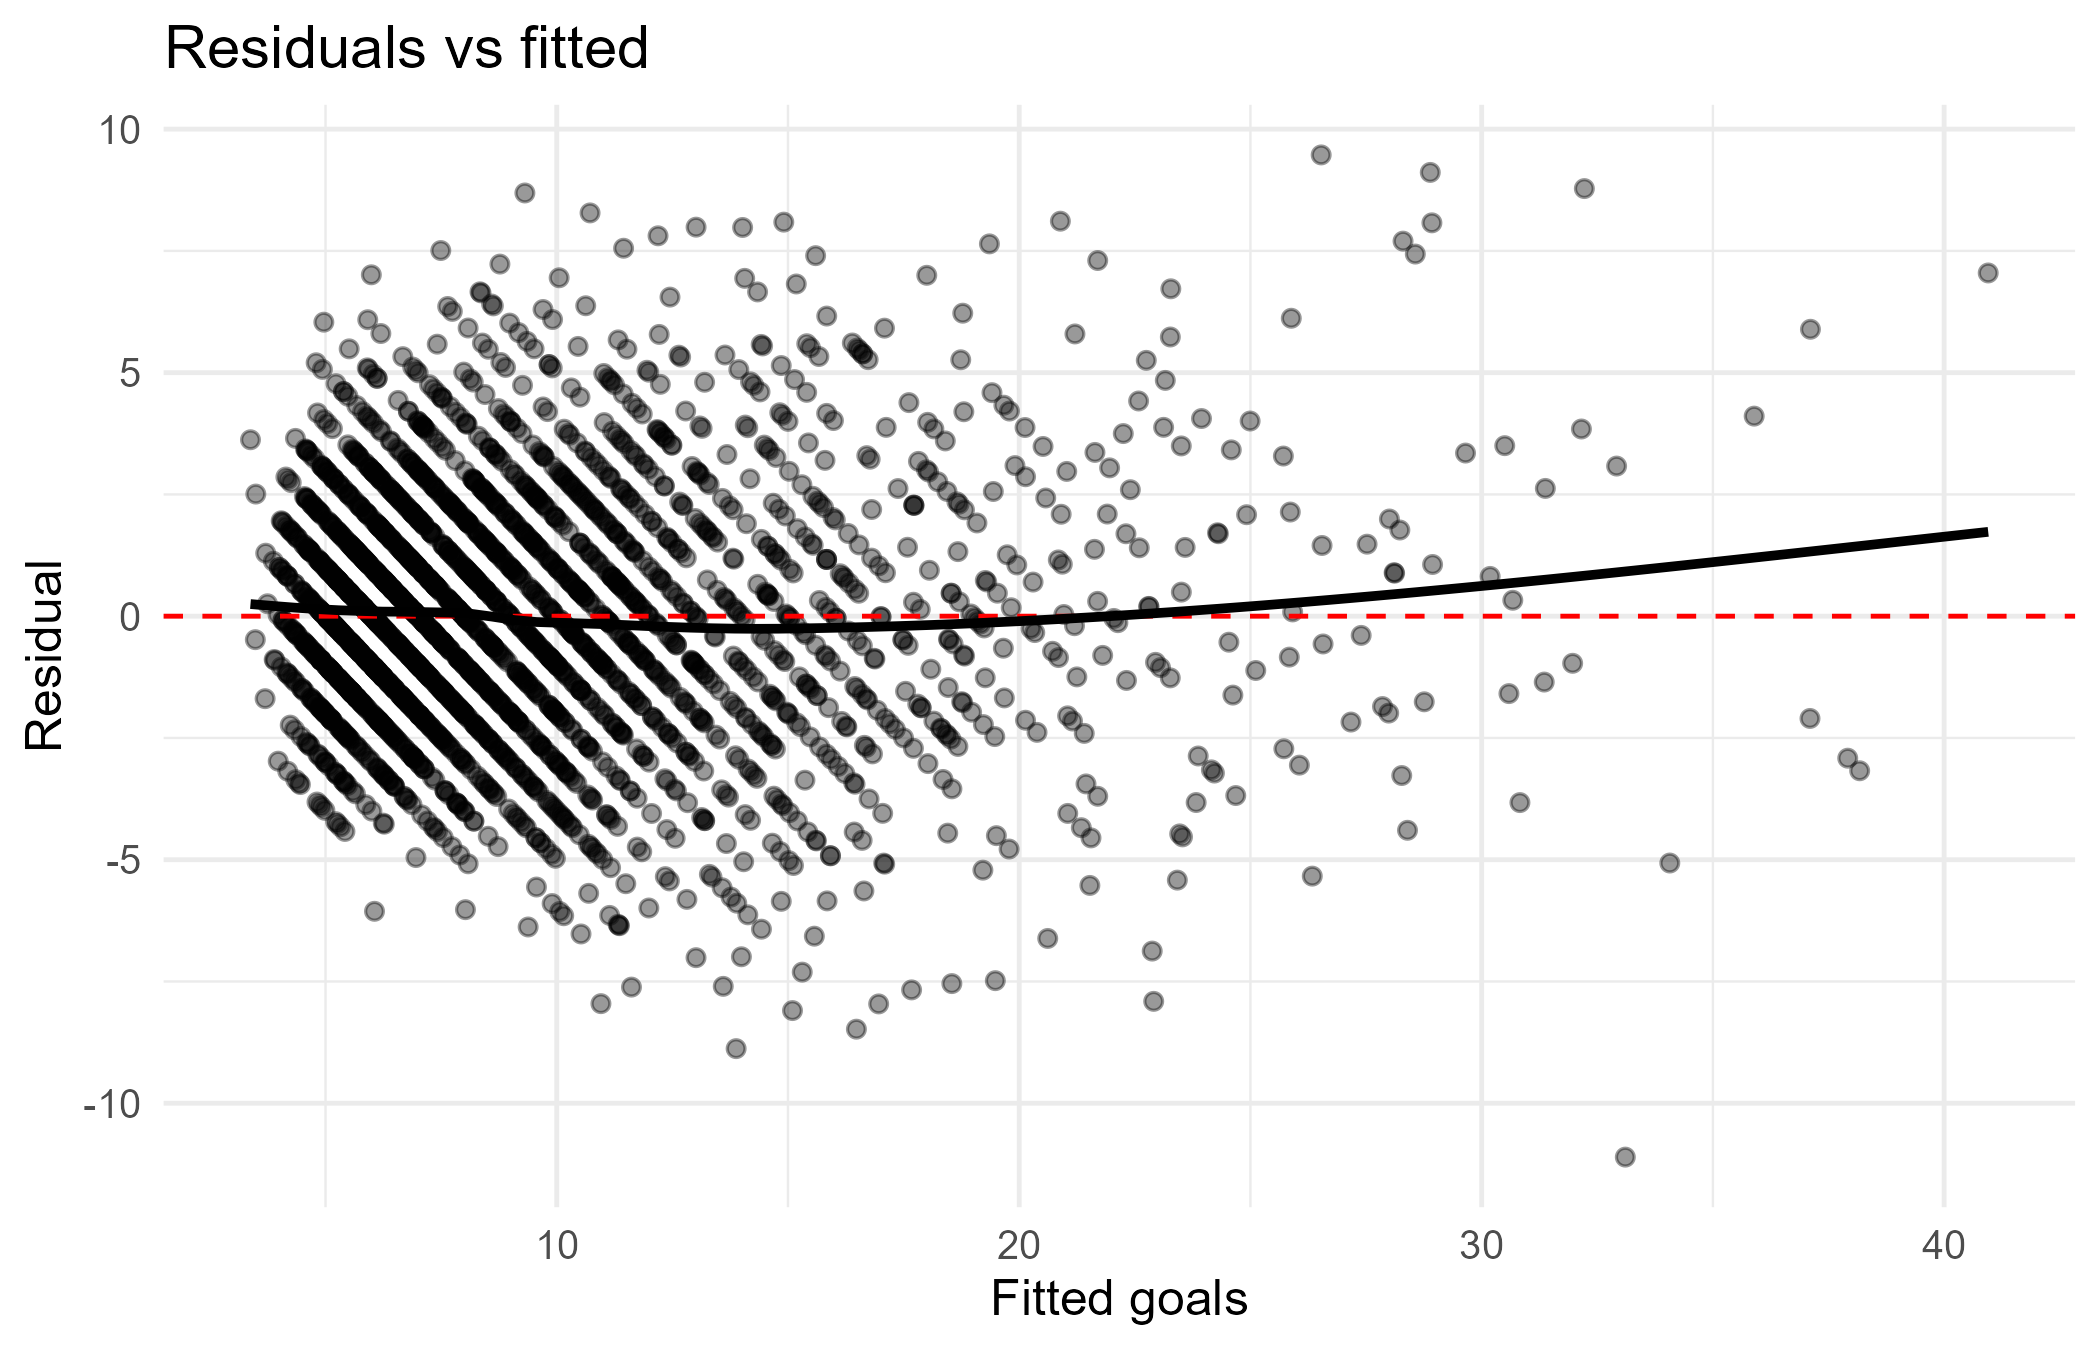
\includegraphics[width=0.48\textwidth]{p2_resid_fitted.png}
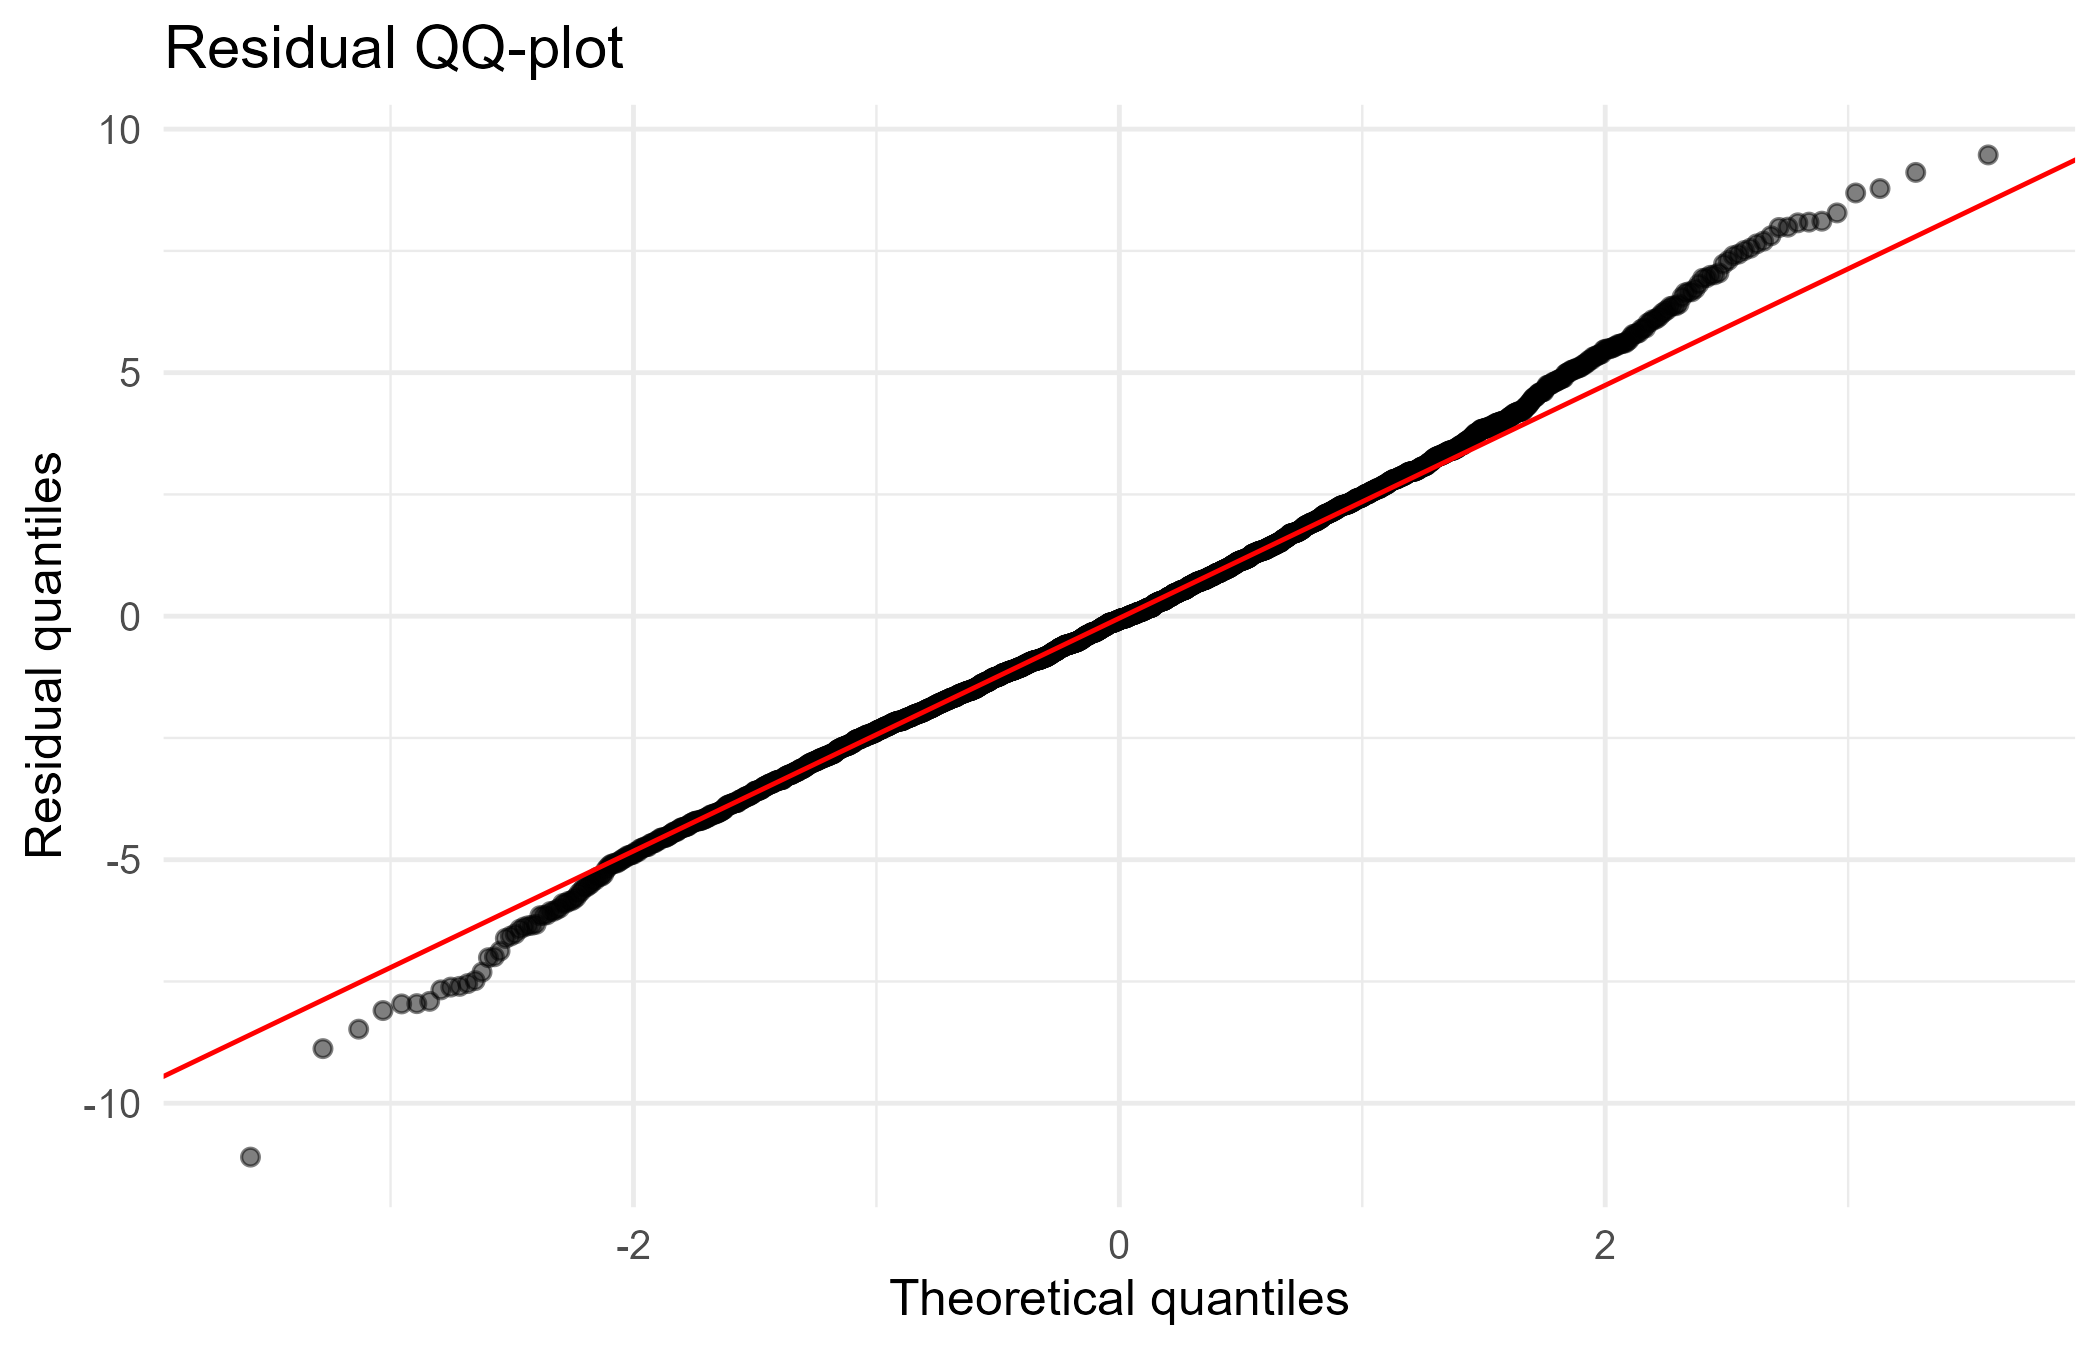
\includegraphics[width=0.48\textwidth]{p2_resid_qq.png}
\caption{Residual diagnostics of the linear model with controls.}
\label{fig:resid}
\end{figure}

\subsection{Robustness to the selection rule}


\begin{table}
\begin{center}
\adjustbox{max width=\textwidth}{\begin{tabular}{l c c c c c}
\toprule
 & (1) xG & (2) + shots & (3) + minutes, midfield & (4) league FE & (5) league + season FE \\
\midrule
(Intercept)             & $3.36^{***}$ & $2.65^{***}$ & $3.25^{***}$ &              &              \\
                        & $(0.35)$     & $(0.41)$     & $(0.43)$     &              &              \\
xg                      & $0.85^{***}$ & $0.76^{***}$ & $0.77^{***}$ & $0.77^{***}$ & $0.80^{***}$ \\
                        & $(0.03)$     & $(0.03)$     & $(0.03)$     & $(0.03)$     & $(0.03)$     \\
shots                   &              & $0.02^{***}$ & $0.03^{***}$ & $0.03^{***}$ & $0.02^{***}$ \\
                        &              & $(0.01)$     & $(0.01)$     & $(0.01)$     & $(0.01)$     \\
time                    &              &              & $-0.00^{*}$  & $-0.00^{*}$  & $-0.00^{*}$  \\
                        &              &              & $(0.00)$     & $(0.00)$     & $(0.00)$     \\
also\_midfield          &              &              & $0.40^{*}$   & $0.37^{*}$   & $0.51^{**}$  \\
                        &              &              & $(0.17)$     & $(0.17)$     & $(0.17)$     \\
\midrule
Num. obs.               & $1136$       & $1136$       & $1136$       & $1136$       & $1136$       \\
R$^2$ (full model)      & $0.74$       & $0.74$       & $0.75$       & $0.75$       & $0.76$       \\
R$^2$ (proj model)      & $$           & $$           & $$           & $0.75$       & $0.75$       \\
Adj. R$^2$ (full model) & $0.74$       & $0.74$       & $0.75$       & $0.75$       & $0.75$       \\
Adj. R$^2$ (proj model) & $$           & $$           & $$           & $0.74$       & $0.75$       \\
Num. groups: league     & $$           & $$           & $$           & $6$          & $6$          \\
Num. groups: season     & $$           & $$           & $$           & $$           & $11$         \\
\bottomrule
\multicolumn{6}{l}{\scriptsize{$^{***}p<0.001$; $^{**}p<0.01$; $^{*}p<0.05$}}
\end{tabular}}
\caption{Goals on xG, shots, minutes and position (goals $\geq$ 10 sample)}
\label{tab:p2_reg_goals_g10}
\end{center}
\end{table}

On the goals $\geq 10$ sample the same specification gives a visibly different picture: the xG slope falls to 0.85 (0.80 with fixed effects) and the intercept rises to 3.4 goals, against a slope of 1.03 and an intercept of $-0.3$ in the xG $\geq 5$ sample. This reproduces the selection effect found in Part 1: conditioning on a high \emph{outcome} flattens the relation between goals and xG, because forwards with low xG enter the sample only if they scored a lot.

\section{Principal components analysis}

Seven standardized metrics are used: goals/xG, xG per 90, shots per 90, xG per shot, xA per 90, key passes per 90 and xG buildup per 90.

\begin{table}

\caption{\label{tab:p2_pca_variance}Variance explained by the principal components}
\centering
\adjustbox{max width=\textwidth}{\begin{tabular}[t]{lrrr}
\toprule
component & eigenvalue & variance\_pct & cumulative\_pct\\
\midrule
PC1 & 2.552 & 36.453 & 36.453\\
PC2 & 1.916 & 27.373 & 63.826\\
PC3 & 1.017 & 14.534 & 78.360\\
PC4 & 0.932 & 13.321 & 91.681\\
PC5 & 0.403 & 5.755 & 97.436\\
\addlinespace
PC6 & 0.159 & 2.275 & 99.712\\
PC7 & 0.020 & 0.288 & 100.000\\
\bottomrule
\end{tabular}}
\end{table}
\begin{table}

\caption{\label{tab:p2_pca_loadings}PCA loadings (first four components)}
\centering
\adjustbox{max width=\textwidth}{\begin{tabular}[t]{lrrrr}
\toprule
variable & PC1 & PC2 & PC3 & PC4\\
\midrule
goals\_xg & 0.128 & -0.131 & 0.533 & -0.826\\
xg\_90 & -0.008 & 0.715 & 0.070 & -0.069\\
shots\_90 & 0.192 & 0.467 & 0.604 & 0.345\\
xg\_per\_shot & -0.204 & 0.487 & -0.500 & -0.434\\
xa\_90 & 0.567 & 0.059 & -0.201 & -0.041\\
\addlinespace
key\_passes\_90 & 0.568 & -0.078 & -0.125 & 0.010\\
xg\_buildup\_90 & 0.511 & 0.086 & -0.198 & -0.062\\
\bottomrule
\end{tabular}}
\end{table}

Three components have eigenvalues above one (Kaiser criterion) and together explain 78\% of the variance (Figure~\ref{fig:scree}). The loadings give a clear interpretation:
\begin{itemize}
\item \textbf{PC1 (36\%) -- creation and involvement:} xA, key passes and xG buildup load around 0.5--0.6.
\item \textbf{PC2 (27\%) -- chance volume and quality:} xG per 90 (0.71), xG per shot (0.49) and shots (0.47).
\item \textbf{PC3 (15\%) -- shot-heavy vs.\ finishing:} shots and goals/xG load positively, xG per shot negatively.
\item \textbf{PC4 (13\%) -- finishing:} dominated by goals/xG (loading $-0.83$), nearly orthogonal to the other dimensions.
\end{itemize}
The fourth component is just below the Kaiser threshold (eigenvalue 0.93) and isolates finishing, which is why goals/xG behaves as an almost independent dimension from chance creation and volume. The biplot (Figure~\ref{fig:biplot}) shows no separation by league.

\begin{figure}[H]
\centering
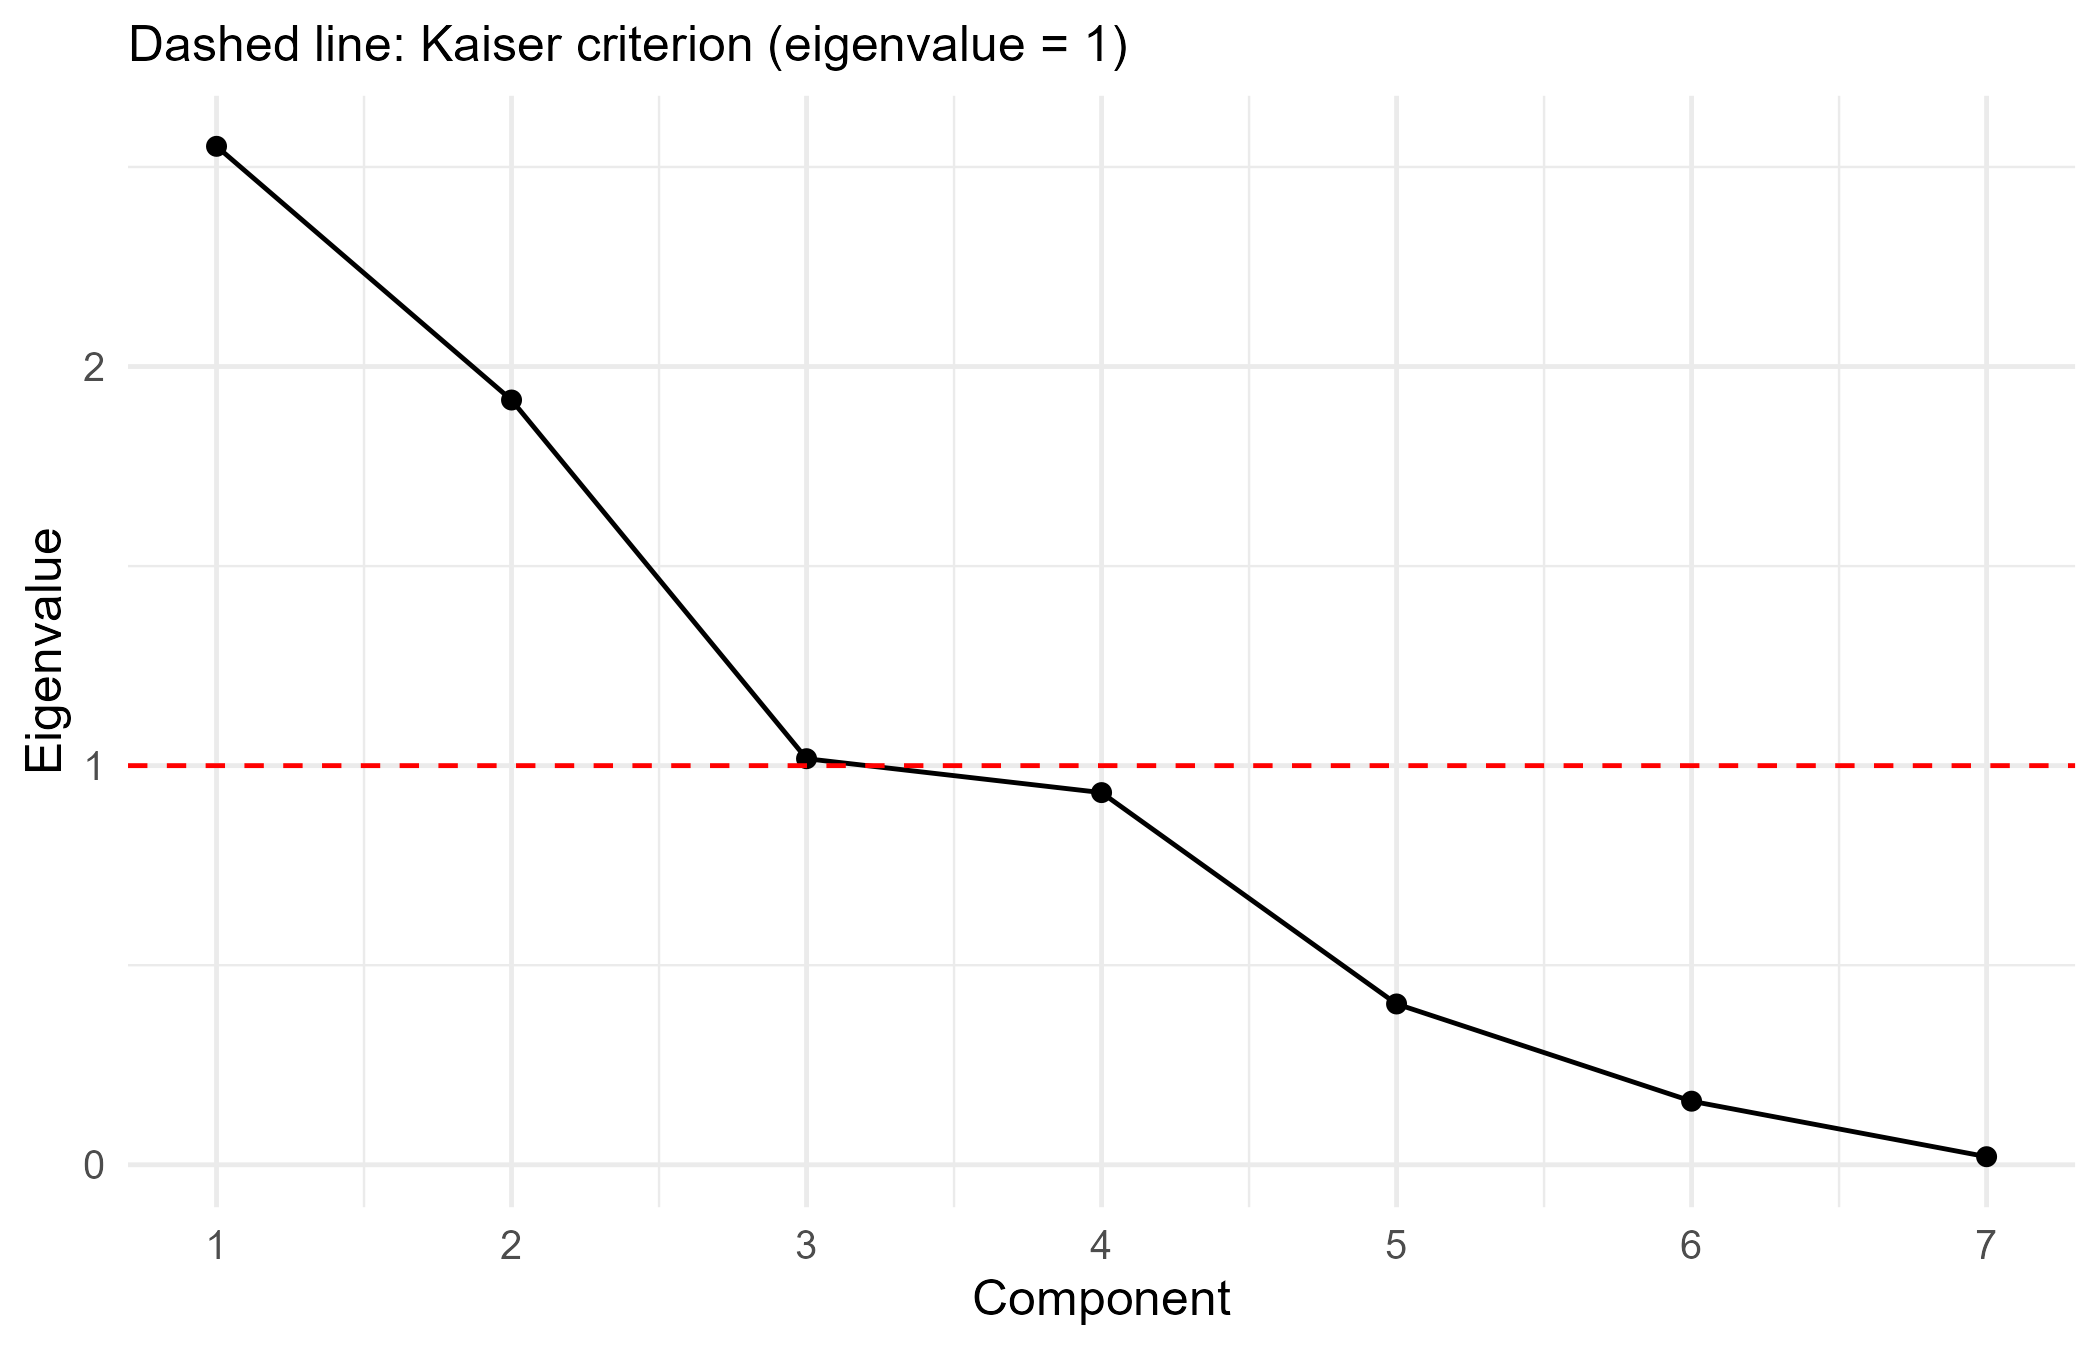
\includegraphics[width=0.6\textwidth]{p2_pca_scree.png}
\caption{Scree plot.}
\label{fig:scree}
\end{figure}

\begin{figure}[H]
\centering
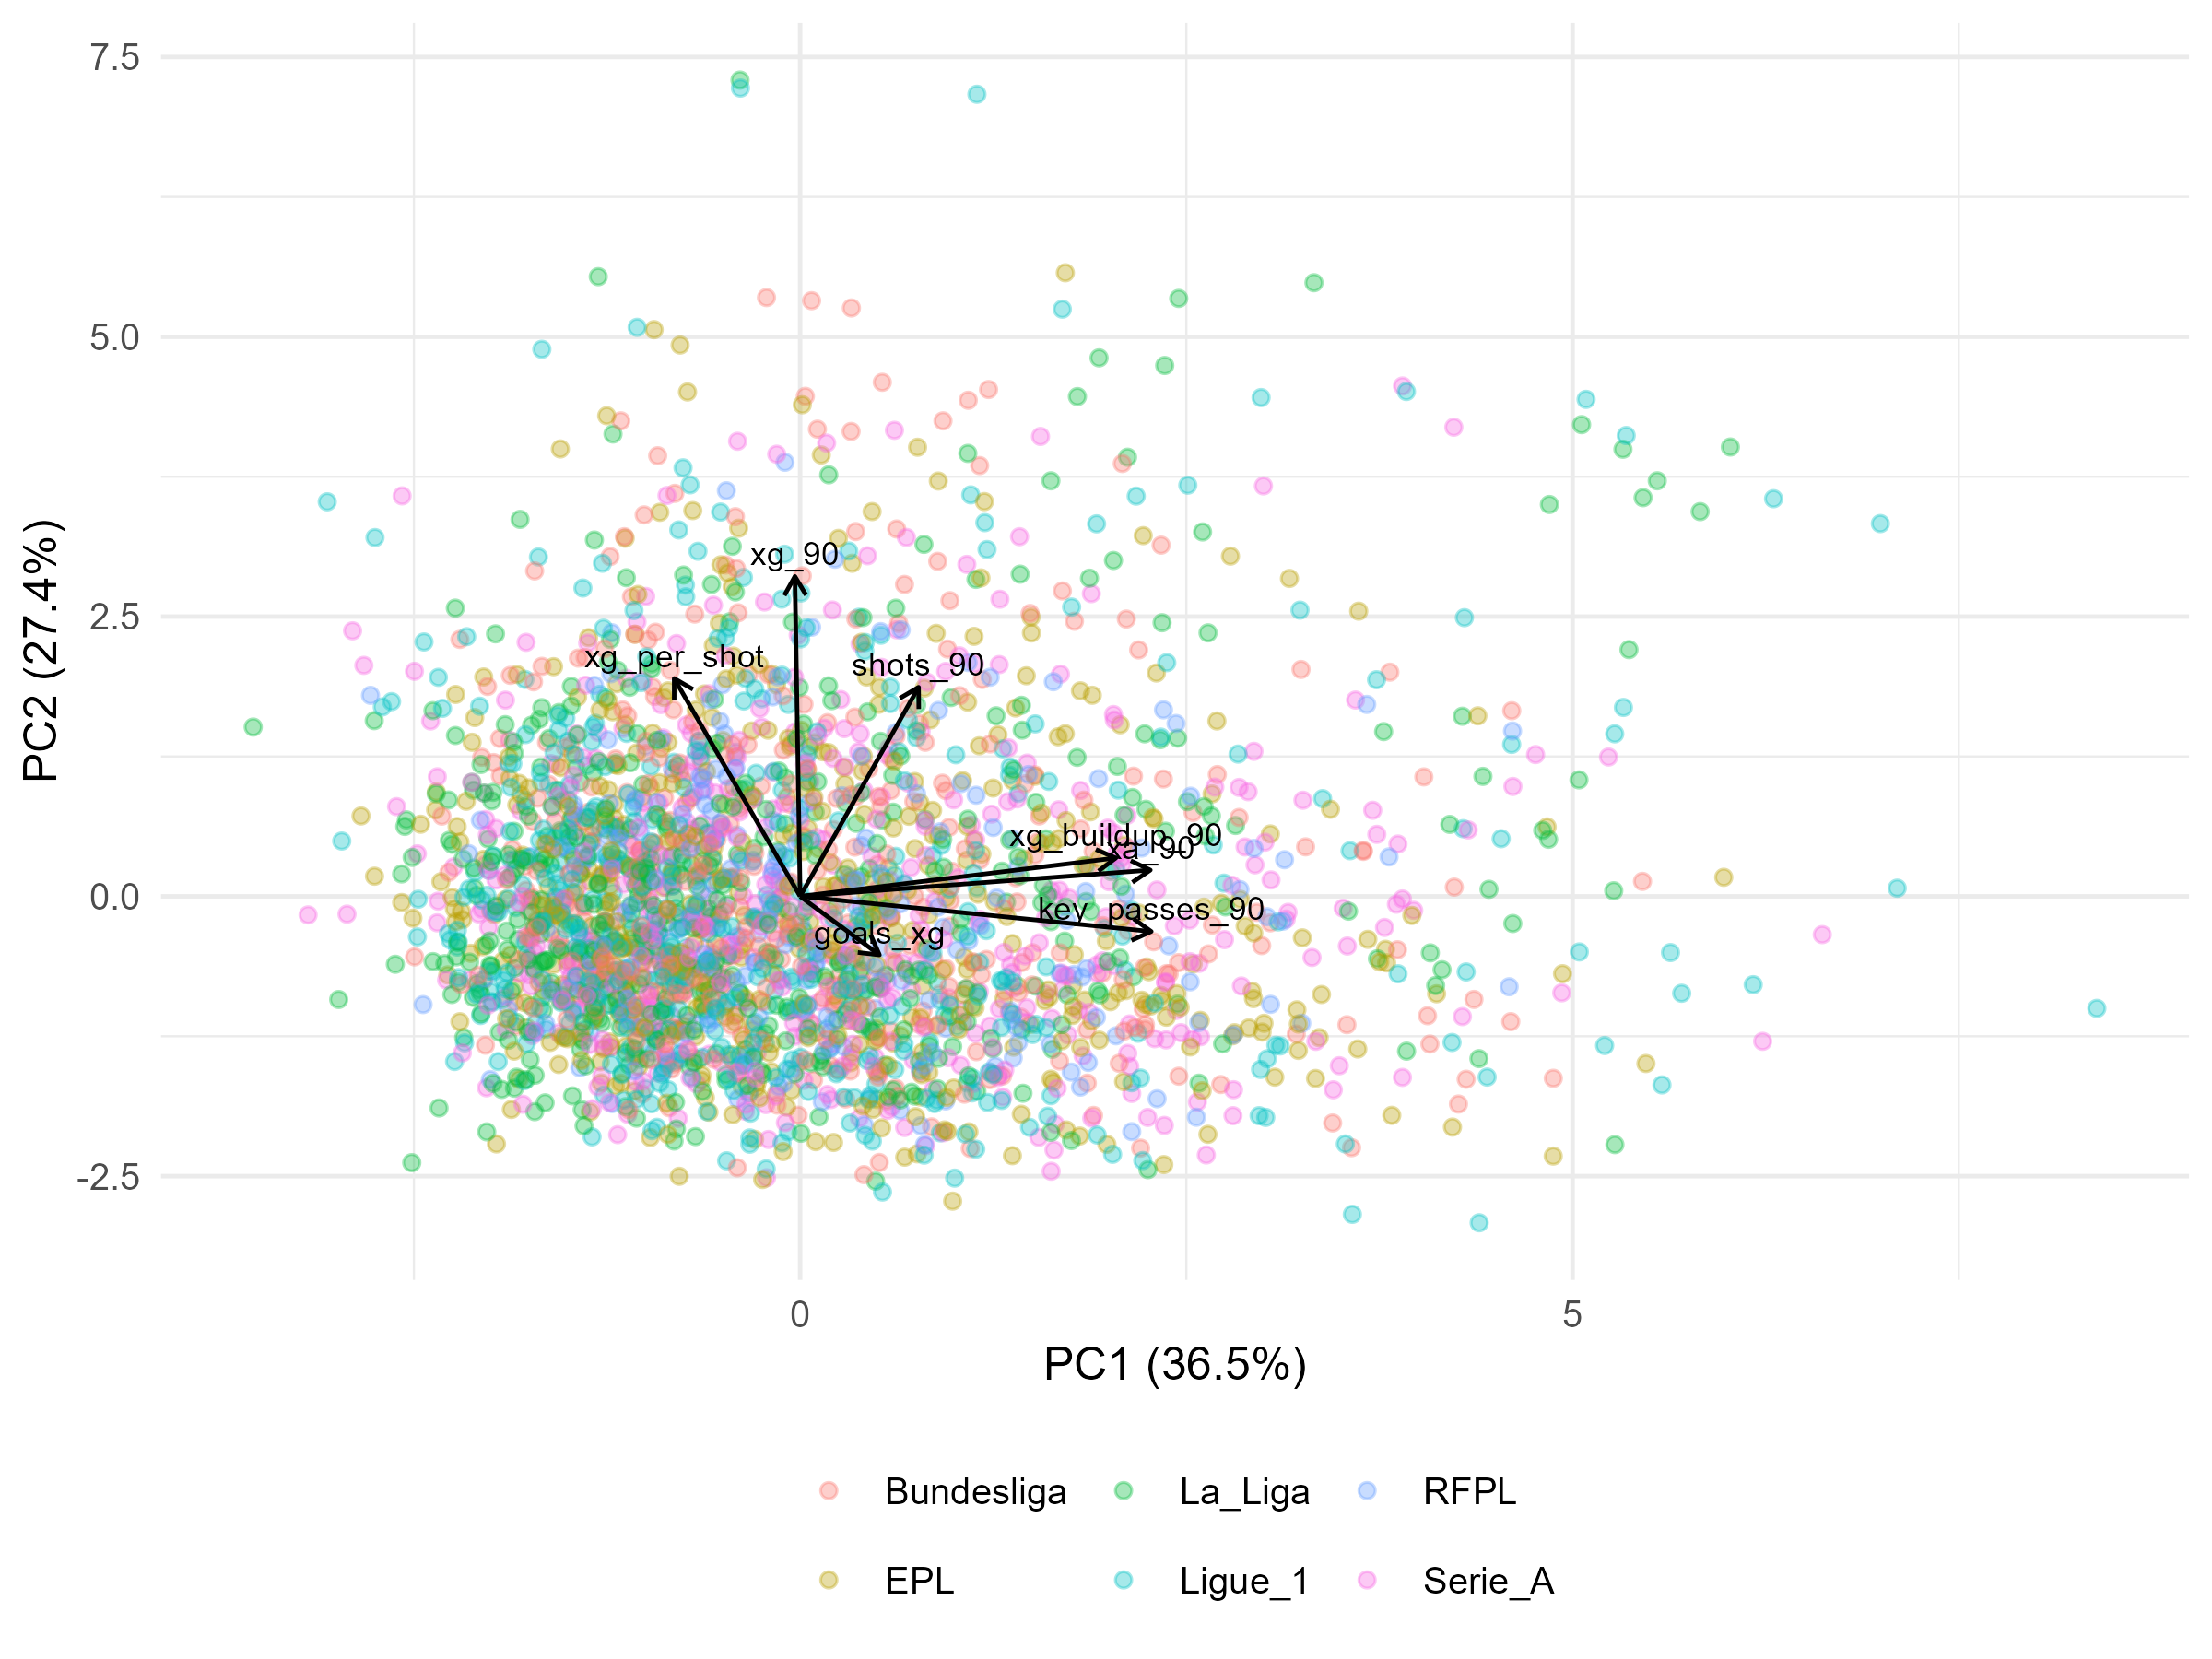
\includegraphics[width=0.8\textwidth]{p2_pca_biplot.png}
\caption{PCA biplot (first two components), colored by league.}
\label{fig:biplot}
\end{figure}

\section{Composite offensive index}

Two indices are built for each player-season. The \emph{equal-weight index} averages three standardized dimensions: finishing (goals/xG), chance volume (xG/90 and shots/90) and creation (xA/90 and key passes/90). The \emph{PCA-weighted index} sums the first three principal components weighted by their variance share, with signs aligned to the equal-weight index since component signs are arbitrary. The two indices agree closely (Pearson $r=0.87$).

\begin{table}

\caption{\label{tab:p2_index_agreement}Agreement between the two composite indices}
\centering
\adjustbox{max width=\textwidth}{\begin{tabular}[t]{lrr}
\toprule
comparison & pearson\_r & spearman\_rho\\
\midrule
Equal-weight index vs PCA-weighted index & 0.871 & 0.845\\
\bottomrule
\end{tabular}}
\end{table}
\begin{table}

\caption{\label{tab:p2_index_equal_ranking}Highest and lowest equal-weight composite index}
\centering
\adjustbox{max width=\textwidth}{\begin{tabular}[t]{lllllrrrr}
\toprule
type & player\_name & season & team\_title & league & goals & xg & goals\_xg & index\_equal\\
\midrule
Top & Lionel Messi & 2018/19 & Barcelona & La\_Liga & 36 & 25.997 & 1.385 & 2.618\\
Top & Cristiano Ronaldo & 2014/15 & Real Madrid & La\_Liga & 48 & 39.309 & 1.221 & 2.443\\
Top & Neymar & 2017/18 & Paris Saint Germain & Ligue\_1 & 19 & 16.538 & 1.149 & 2.373\\
Top & Lionel Messi & 2016/17 & Barcelona & La\_Liga & 37 & 26.885 & 1.376 & 2.327\\
Top & Kylian Mbappe-Lottin & 2019/20 & Paris Saint Germain & Ligue\_1 & 18 & 16.572 & 1.086 & 2.302\\
\addlinespace
Top & Luis Muriel & 2019/20 & Atalanta & Serie\_A & 18 & 13.169 & 1.367 & 2.280\\
Top & Luis Muriel & 2020/21 & Atalanta & Serie\_A & 22 & 16.692 & 1.318 & 2.242\\
Top & Ángel Di María & 2015/16 & Paris Saint Germain & Ligue\_1 & 10 & 6.792 & 1.472 & 2.234\\
Top & Gareth Bale & 2015/16 & Real Madrid & La\_Liga & 19 & 10.659 & 1.783 & 2.222\\
Top & Lionel Messi & 2017/18 & Barcelona & La\_Liga & 34 & 28.946 & 1.175 & 2.203\\
\addlinespace
Bottom & Miguel De la Fuente & 2024/25 & Leganes & La\_Liga & 1 & 5.791 & 0.173 & -1.682\\
Bottom & Mathew Leckie & 2016/17 & Ingolstadt & Bundesliga & 0 & 5.087 & 0.000 & -1.647\\
Bottom & Cameron Archer & 2024/25 & Southampton & EPL & 2 & 6.928 & 0.289 & -1.463\\
Bottom & Mateus Fernandes & 2024/25 & Southampton & EPL & 2 & 5.011 & 0.399 & -1.418\\
Bottom & Joelinton & 2019/20 & Newcastle United & EPL & 2 & 6.031 & 0.332 & -1.411\\
\addlinespace
Bottom & Hugo Duro & 2022/23 & Valencia & La\_Liga & 1 & 5.360 & 0.187 & -1.406\\
Bottom & Neal Maupay & 2022/23 & Everton & EPL & 1 & 5.435 & 0.184 & -1.366\\
Bottom & Nemanja Maksimovic & 2023/24 & Getafe & La\_Liga & 4 & 5.083 & 0.787 & -1.360\\
Bottom & Hanno Behrens & 2018/19 & Nuernberg & Bundesliga & 4 & 7.998 & 0.500 & -1.356\\
Bottom & Dan Ndoye & 2023/24 & Bologna & Serie\_A & 1 & 6.087 & 0.164 & -1.342\\
\bottomrule
\end{tabular}}
\end{table}
\begin{table}

\caption{\label{tab:p2_index_career_top15}Top 15 forwards by mean composite index (3+ seasons)}
\centering
\adjustbox{max width=\textwidth}{\begin{tabular}[t]{rlrrrrrr}
\toprule
id & player\_name & seasons & goals & xg & index\_equal & index\_pca & goals\_xg\\
\midrule
2097 & Lionel Messi & 9 & 253 & 219.893 & 1.863 & 3.661 & 1.151\\
2099 & Neymar & 9 & 140 & 143.003 & 1.450 & 2.947 & 0.979\\
2371 & Cristiano Ronaldo & 7 & 215 & 209.905 & 1.446 & 2.874 & 1.024\\
3423 & Kylian Mbappe-Lottin & 9 & 222 & 196.098 & 1.420 & 2.401 & 1.132\\
1384 & Dries Mertens & 6 & 91 & 74.143 & 1.228 & 1.660 & 1.227\\
\addlinespace
1426 & Josip Ilicic & 5 & 49 & 42.768 & 1.216 & 2.274 & 1.146\\
3553 & Ángel Di María & 7 & 57 & 54.662 & 1.180 & 2.233 & 1.043\\
1741 & Zlatan Ibrahimovic & 6 & 107 & 96.967 & 1.063 & 1.974 & 1.103\\
1229 & Luis Muriel & 6 & 73 & 61.626 & 0.995 & 1.550 & 1.185\\
2815 & Quincy Promes & 6 & 84 & 67.025 & 0.987 & 1.282 & 1.253\\
\addlinespace
701 & Eden Hazard & 3 & 44 & 31.544 & 0.965 & 1.088 & 1.395\\
536 & Dimitri Payet & 7 & 53 & 47.717 & 0.941 & 1.249 & 1.111\\
392 & Arjen Robben & 3 & 22 & 17.061 & 0.933 & 1.560 & 1.289\\
619 & Sergio Agüero & 6 & 128 & 122.095 & 0.917 & 1.705 & 1.048\\
555 & Memphis Depay & 5 & 67 & 61.600 & 0.912 & 1.508 & 1.088\\
\bottomrule
\end{tabular}}
\end{table}

The rankings are plausible: Messi (2018/19, 2016/17, 2017/18) and Cristiano Ronaldo (2014/15) lead the single-season ranking, and over three or more seasons Messi, Neymar, Cristiano Ronaldo and Mbappe lead. The bottom of the ranking is populated by low-minutes forwards with almost no goals. A caveat is that the index mixes a very noisy component (goals/xG) with stable ones, which matters for prediction, as discussed next.

\section{Persistence: skill or luck?}

If goals/xG measured stable finishing skill, a forward's ratio in season $t$ should predict the ratio in season $t+1$. Using 1{,}407 consecutive player-season pairs (532 players), I compute correlations and slopes of each metric between seasons.

\begin{table}

\caption{\label{tab:p2_persistence}Year-to-year persistence of each metric (season t vs t+1)}
\centering
\adjustbox{max width=\textwidth}{\begin{tabular}[t]{lrrrrrrr}
\toprule
variable & n\_pairs & pearson\_r & r\_ci\_low & r\_ci\_high & spearman\_rho & slope & slope\_se\\
\midrule
goals\_xg & 1407 & 0.089 & 0.037 & 0.141 & 0.089 & 0.090 & 0.027\\
npg\_npxg & 1407 & 0.075 & 0.023 & 0.127 & 0.078 & 0.077 & 0.027\\
xg\_90 & 1407 & 0.642 & 0.611 & 0.672 & 0.602 & 0.650 & 0.021\\
shots\_90 & 1407 & 0.687 & 0.659 & 0.714 & 0.626 & 0.683 & 0.019\\
xg\_per\_shot & 1407 & 0.606 & 0.572 & 0.638 & 0.581 & 0.628 & 0.022\\
\addlinespace
xa\_90 & 1407 & 0.610 & 0.576 & 0.642 & 0.566 & 0.629 & 0.022\\
key\_passes\_90 & 1407 & 0.752 & 0.729 & 0.774 & 0.689 & 0.778 & 0.018\\
goals\_90 & 1407 & 0.511 & 0.471 & 0.549 & 0.439 & 0.516 & 0.023\\
\bottomrule
\end{tabular}}
\end{table}

\begin{figure}[H]
\centering
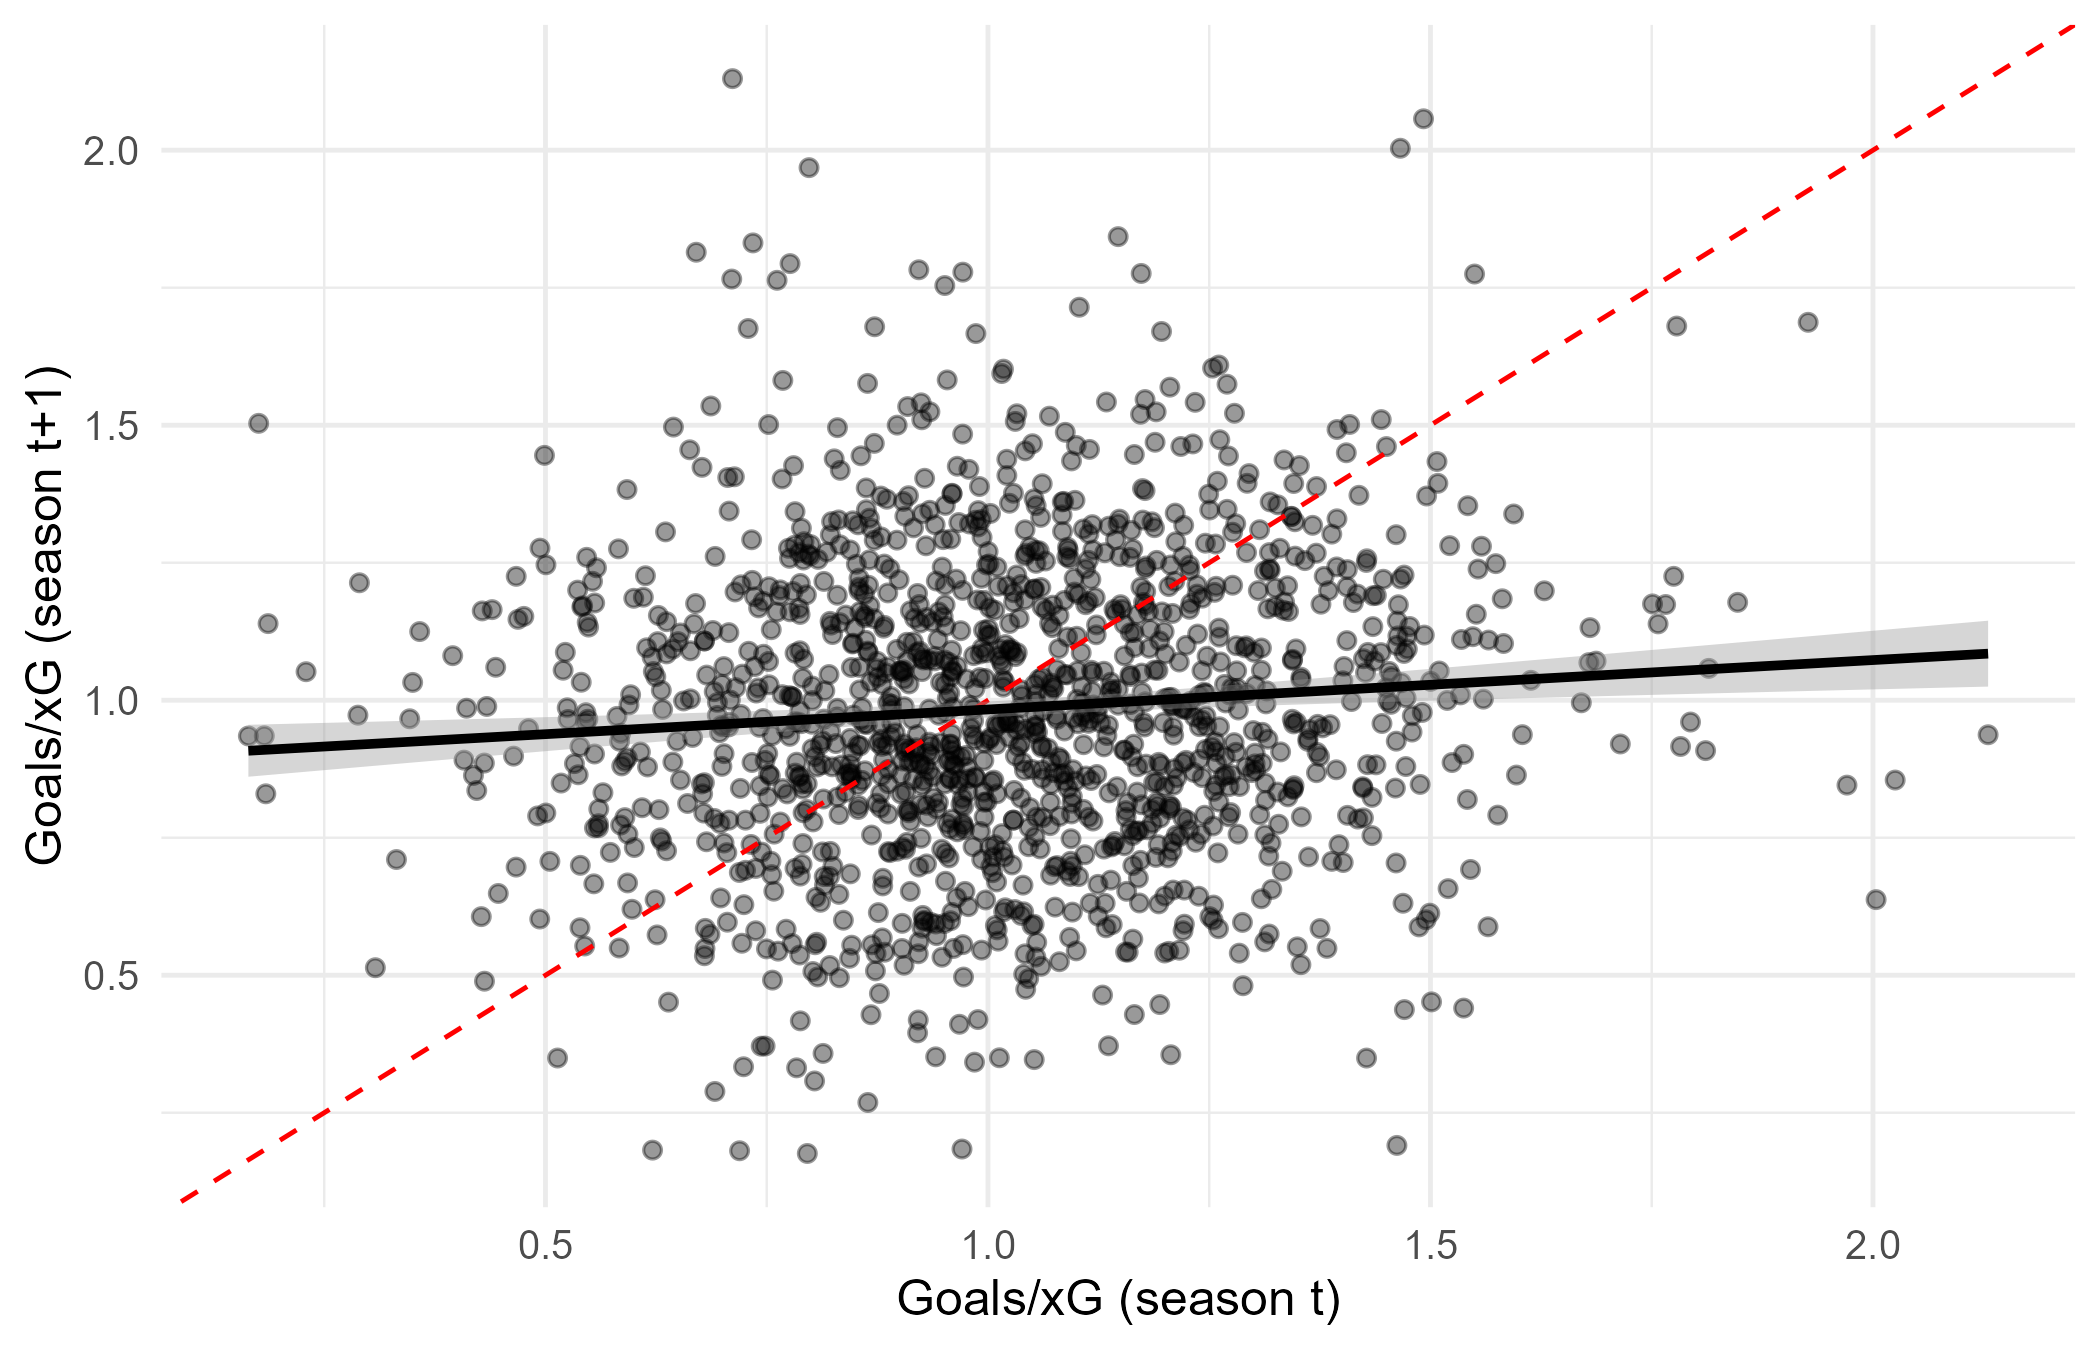
\includegraphics[width=0.48\textwidth]{p2_persistence_goals_xg.png}
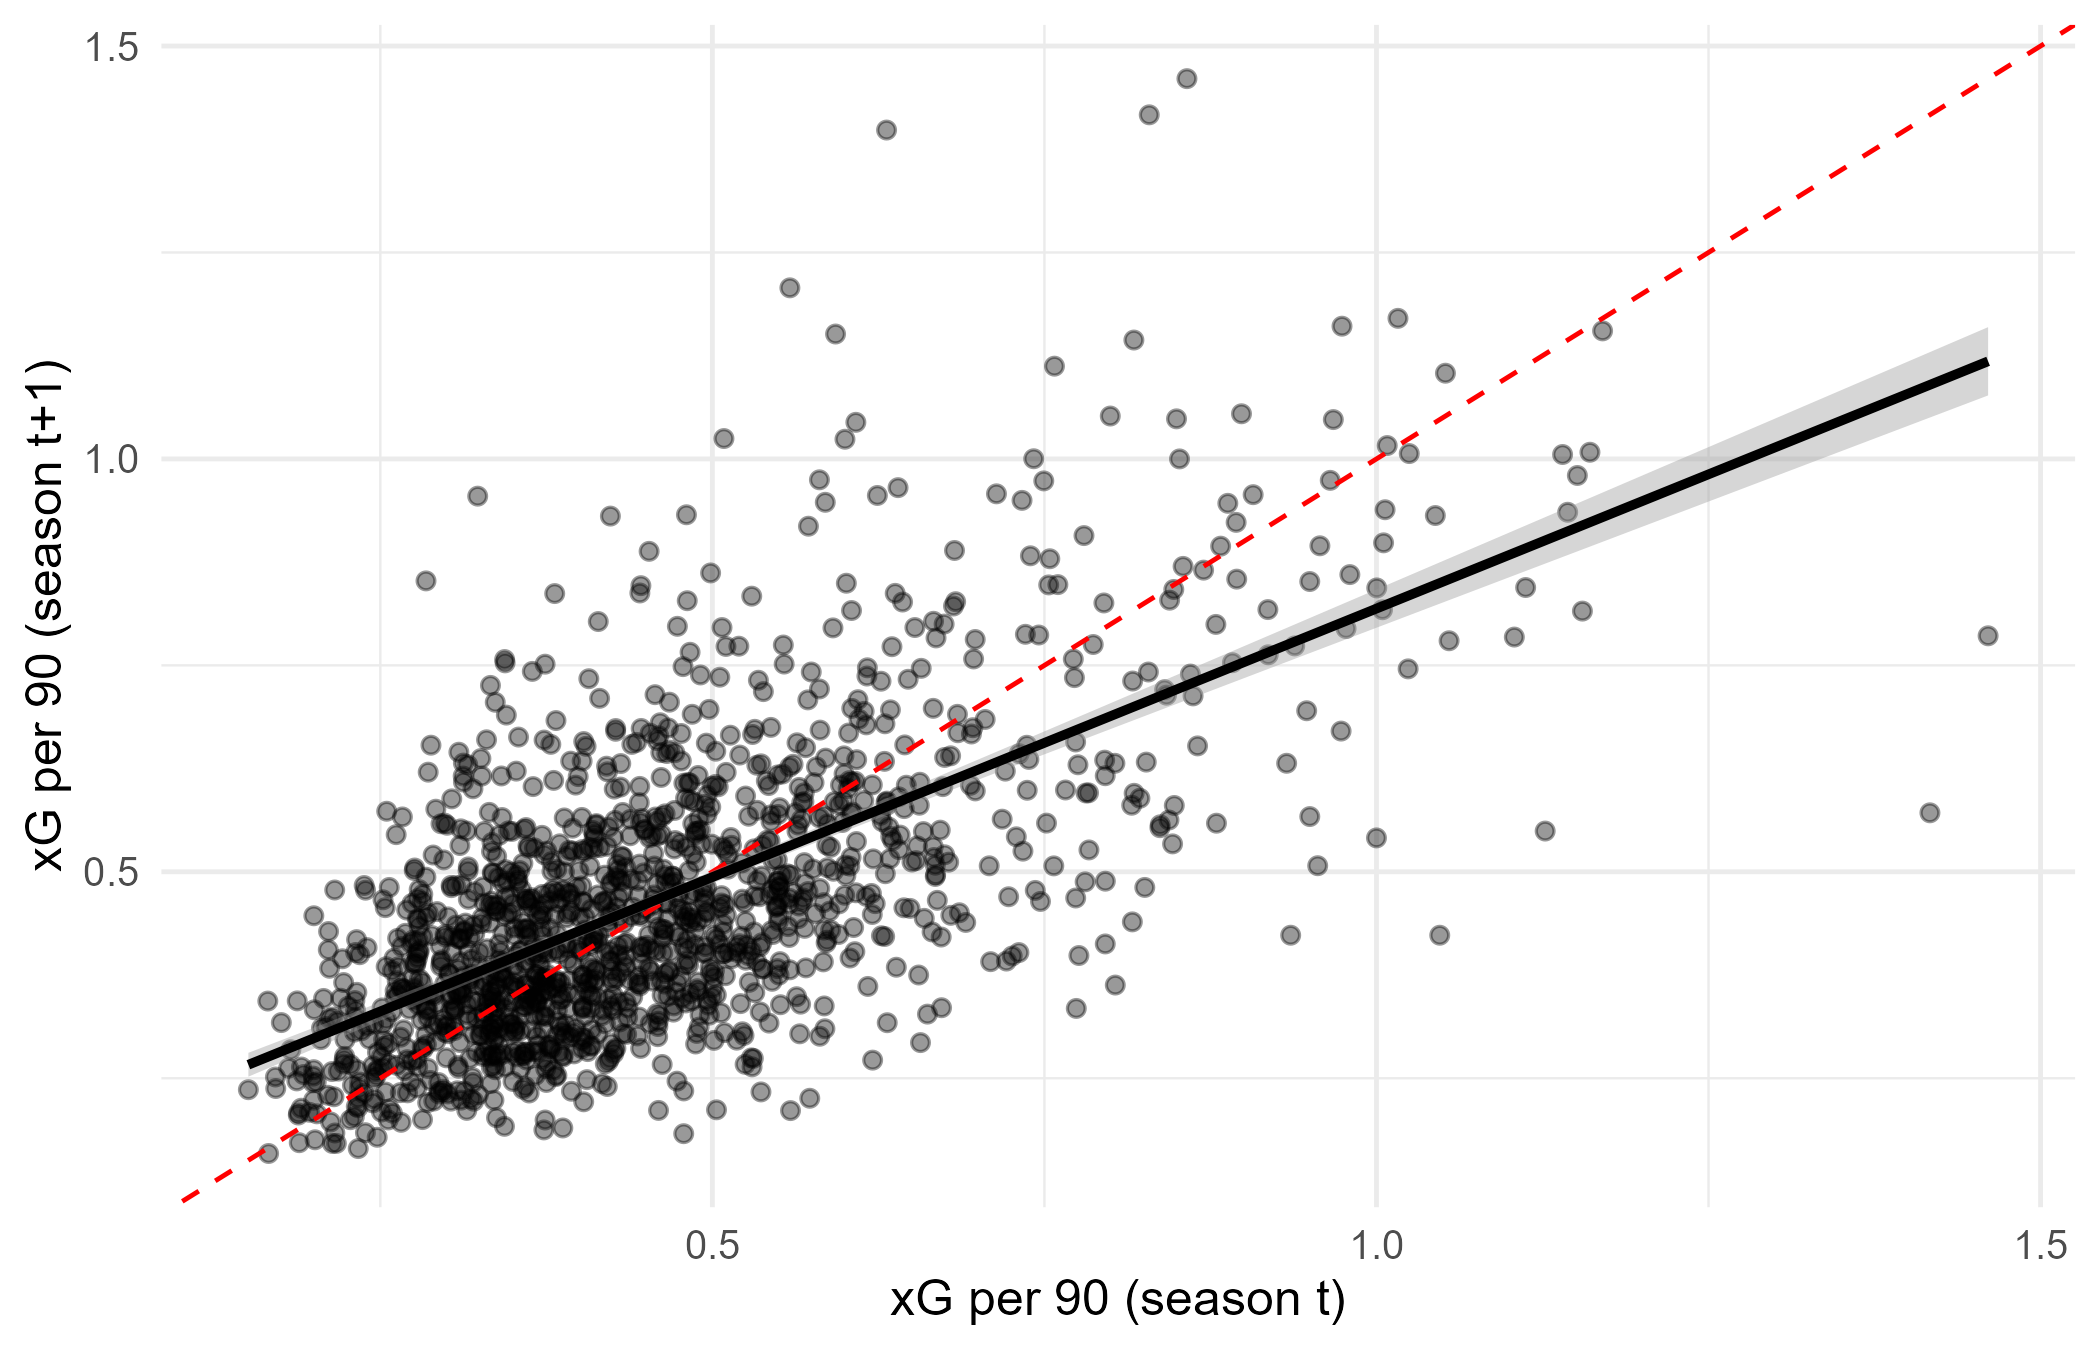
\includegraphics[width=0.48\textwidth]{p2_persistence_xg_90.png}
\caption{Season-to-season persistence of goals/xG (left) and xG per 90 (right). Dashed line: 45 degrees.}
\label{fig:persistence}
\end{figure}

The year-to-year correlation of goals/xG is only 0.09 (95\% CI 0.04--0.14), against 0.64 for xG per 90, 0.69 for shots per 90 and 0.75 for key passes per 90. About 91\% of the deviation of a forward's ratio from the mean disappears the next season, so most of a single-season goals/xG is noise (or luck), with at most a small stable skill component. Forwards' ability to \emph{get into} good positions is far more persistent than their conversion.

The same conclusion appears in prediction (Table~\ref{tab:p2_reg_next_season_goals}): next-season goals per 90 are explained only 0.3\% by current goals/xG, but 28\% by current xG per 90. Adding goals/xG to xG per 90 raises $R^2$ only from 0.28 to 0.29, although its coefficient is statistically significant, which is evidence of a small but real finishing skill. Both composite indices predict less than xG per 90 alone ($R^2$ of 0.14 and 0.17) because they carry the noisy finishing component.


\begin{table}
\begin{center}
\adjustbox{max width=\textwidth}{\begin{tabular}{l c c c c c c}
\toprule
 & (1) goals/xG & (2) xG/90 & (3) goals/xG + xG/90 & (4) + shots/90, xA/90 & (5) equal-weight index & (6) PCA index \\
\midrule
(Intercept)             & $0.41^{***}$ & $0.17^{***}$ & $0.08^{**}$  & $0.03$       & $0.44^{***}$ & $0.44^{***}$ \\
                        & $(0.02)$     & $(0.02)$     & $(0.03)$     & $(0.03)$     & $(0.01)$     & $(0.01)$     \\
goals\_xg\_t            & $0.05^{*}$   &              & $0.08^{***}$ & $0.07^{***}$ &              &              \\
                        & $(0.02)$     &              & $(0.02)$     & $(0.02)$     &              &              \\
xg\_90\_t               &              & $0.63^{***}$ & $0.64^{***}$ & $0.56^{***}$ &              &              \\
                        &              & $(0.04)$     & $(0.04)$     & $(0.04)$     &              &              \\
shots\_90\_t            &              &              &              & $0.02^{**}$  &              &              \\
                        &              &              &              & $(0.01)$     &              &              \\
xa\_90\_t               &              &              &              & $0.16^{*}$   &              &              \\
                        &              &              &              & $(0.07)$     &              &              \\
index\_equal\_t         &              &              &              &              & $0.14^{***}$ &              \\
                        &              &              &              &              & $(0.02)$     &              \\
index\_pca\_t           &              &              &              &              &              & $0.09^{***}$ \\
                        &              &              &              &              &              & $(0.01)$     \\
\midrule
Num. obs.               & $1407$       & $1407$       & $1407$       & $1407$       & $1407$       & $1407$       \\
R$^2$ (full model)      & $0.00$       & $0.28$       & $0.29$       & $0.30$       & $0.14$       & $0.17$       \\
R$^2$ (proj model)      & $$           & $$           & $$           & $$           & $$           & $$           \\
Adj. R$^2$ (full model) & $0.00$       & $0.28$       & $0.29$       & $0.30$       & $0.14$       & $0.17$       \\
Adj. R$^2$ (proj model) & $$           & $$           & $$           & $$           & $$           & $$           \\
\bottomrule
\multicolumn{7}{l}{\scriptsize{$^{***}p<0.001$; $^{**}p<0.01$; $^{*}p<0.05$}}
\end{tabular}}
\caption{Predicting next-season goals per 90 with current-season metrics}
\label{tab:p2_reg_next_season_goals}
\end{center}
\end{table}
\begin{table}

\caption{\label{tab:p2_prediction_fit}Out-of-season fit of the prediction models}
\centering
\adjustbox{max width=\textwidth}{\begin{tabular}[t]{lrr}
\toprule
model & r2 & n\\
\midrule
(1) goals/xG & 0.003 & 1407\\
(2) xG/90 & 0.281 & 1407\\
(3) goals/xG + xG/90 & 0.293 & 1407\\
(4) + shots/90, xA/90 & 0.303 & 1407\\
(5) equal-weight index & 0.141 & 1407\\
\addlinespace
(6) PCA index & 0.166 & 1407\\
\bottomrule
\end{tabular}}
\end{table}

\section{Goalkeepers}

\subsection{Design}

Understat's player data contain no post-shot xG or saves, so the goalkeeper effect is proxied at the team level by goals conceded relative to expected goals against, $\text{ga}/\text{xGA}$ (a value below one means the team conceded less than the shots' quality implied). The measure mixes goalkeeping with defensive quality after the shot, so it is a proxy, not a pure shot-stopping metric.

To test whether \emph{elite} goalkeepers concede fewer goals than expected without circularity, ``elite'' is defined out of sample: a goalkeeper-season is elite if the goalkeeper's $\text{ga}/\text{xGA}$ in \emph{all other} seasons is in the lowest quartile (requiring at least two other seasons). The tested season is therefore never used to select the group. This leaves 858 eligible seasons, 215 of them elite.

\subsection{Results}

\begin{table}

\caption{\label{tab:p2_gk_groups}Elite vs other goalkeepers}
\centering
\adjustbox{max width=\textwidth}{\begin{tabular}[t]{lrrrrrrr}
\toprule
elite\_label & n & mean\_ga\_xga & median\_ga\_xga & sd\_ga\_xga & mean\_goals\_prevented & mean\_xga\_90 & mean\_prior\_ratio\\
\midrule
Other & 643 & 0.998 & 0.990 & 0.139 & 0.173 & 1.336 & 1.020\\
Elite (prior ratio, bottom quartile) & 215 & 0.962 & 0.953 & 0.129 & 1.903 & 1.288 & 0.891\\
\bottomrule
\end{tabular}}
\end{table}
\begin{table}

\caption{\label{tab:p2_gk_tests}Goalkeeper hypothesis tests}
\centering
\adjustbox{max width=\textwidth}{\begin{tabular}[t]{lrl}
\toprule
hypothesis & statistic & p\_value\\
\midrule
Elite: mean ga/xGA < 1 (t-test) & -4.308 & < 1e-04\\
Elite: median ga/xGA < 1 (Wilcoxon) & 7951.000 & < 1e-04\\
Other: mean ga/xGA = 1 (t-test) & -0.295 & 0.767858\\
Elite mean < other mean (Welch) & -3.502 & 0.000257\\
Elite distribution < other (Wilcoxon) & 59220.000 & 0.000823\\
\addlinespace
xGA per match: elite = other (Welch) & -2.066 & 0.039519\\
\bottomrule
\end{tabular}}
\end{table}

Elite goalkeepers conceded 3.8\% fewer goals than their xGA in the tested season (mean ratio 0.962, one-sided $p<0.001$), whereas other goalkeepers are indistinguishable from one (0.998, $p=0.77$). The difference between the groups is significant (Welch $p<0.001$, Wilcoxon $p<0.001$); Figure~\ref{fig:gkbox} shows the shift. In terms of goals, the elite group prevented about 1.9 goals per season above expectation versus 0.2 for the others.

The prior ratio of the elite group averaged 0.89 while their realized ratio is 0.96: roughly 30\% of the previous advantage carries over. This regression toward the mean is the same phenomenon as in the forwards' case and is exactly what an out-of-sample test should show.

\begin{figure}[H]
\centering
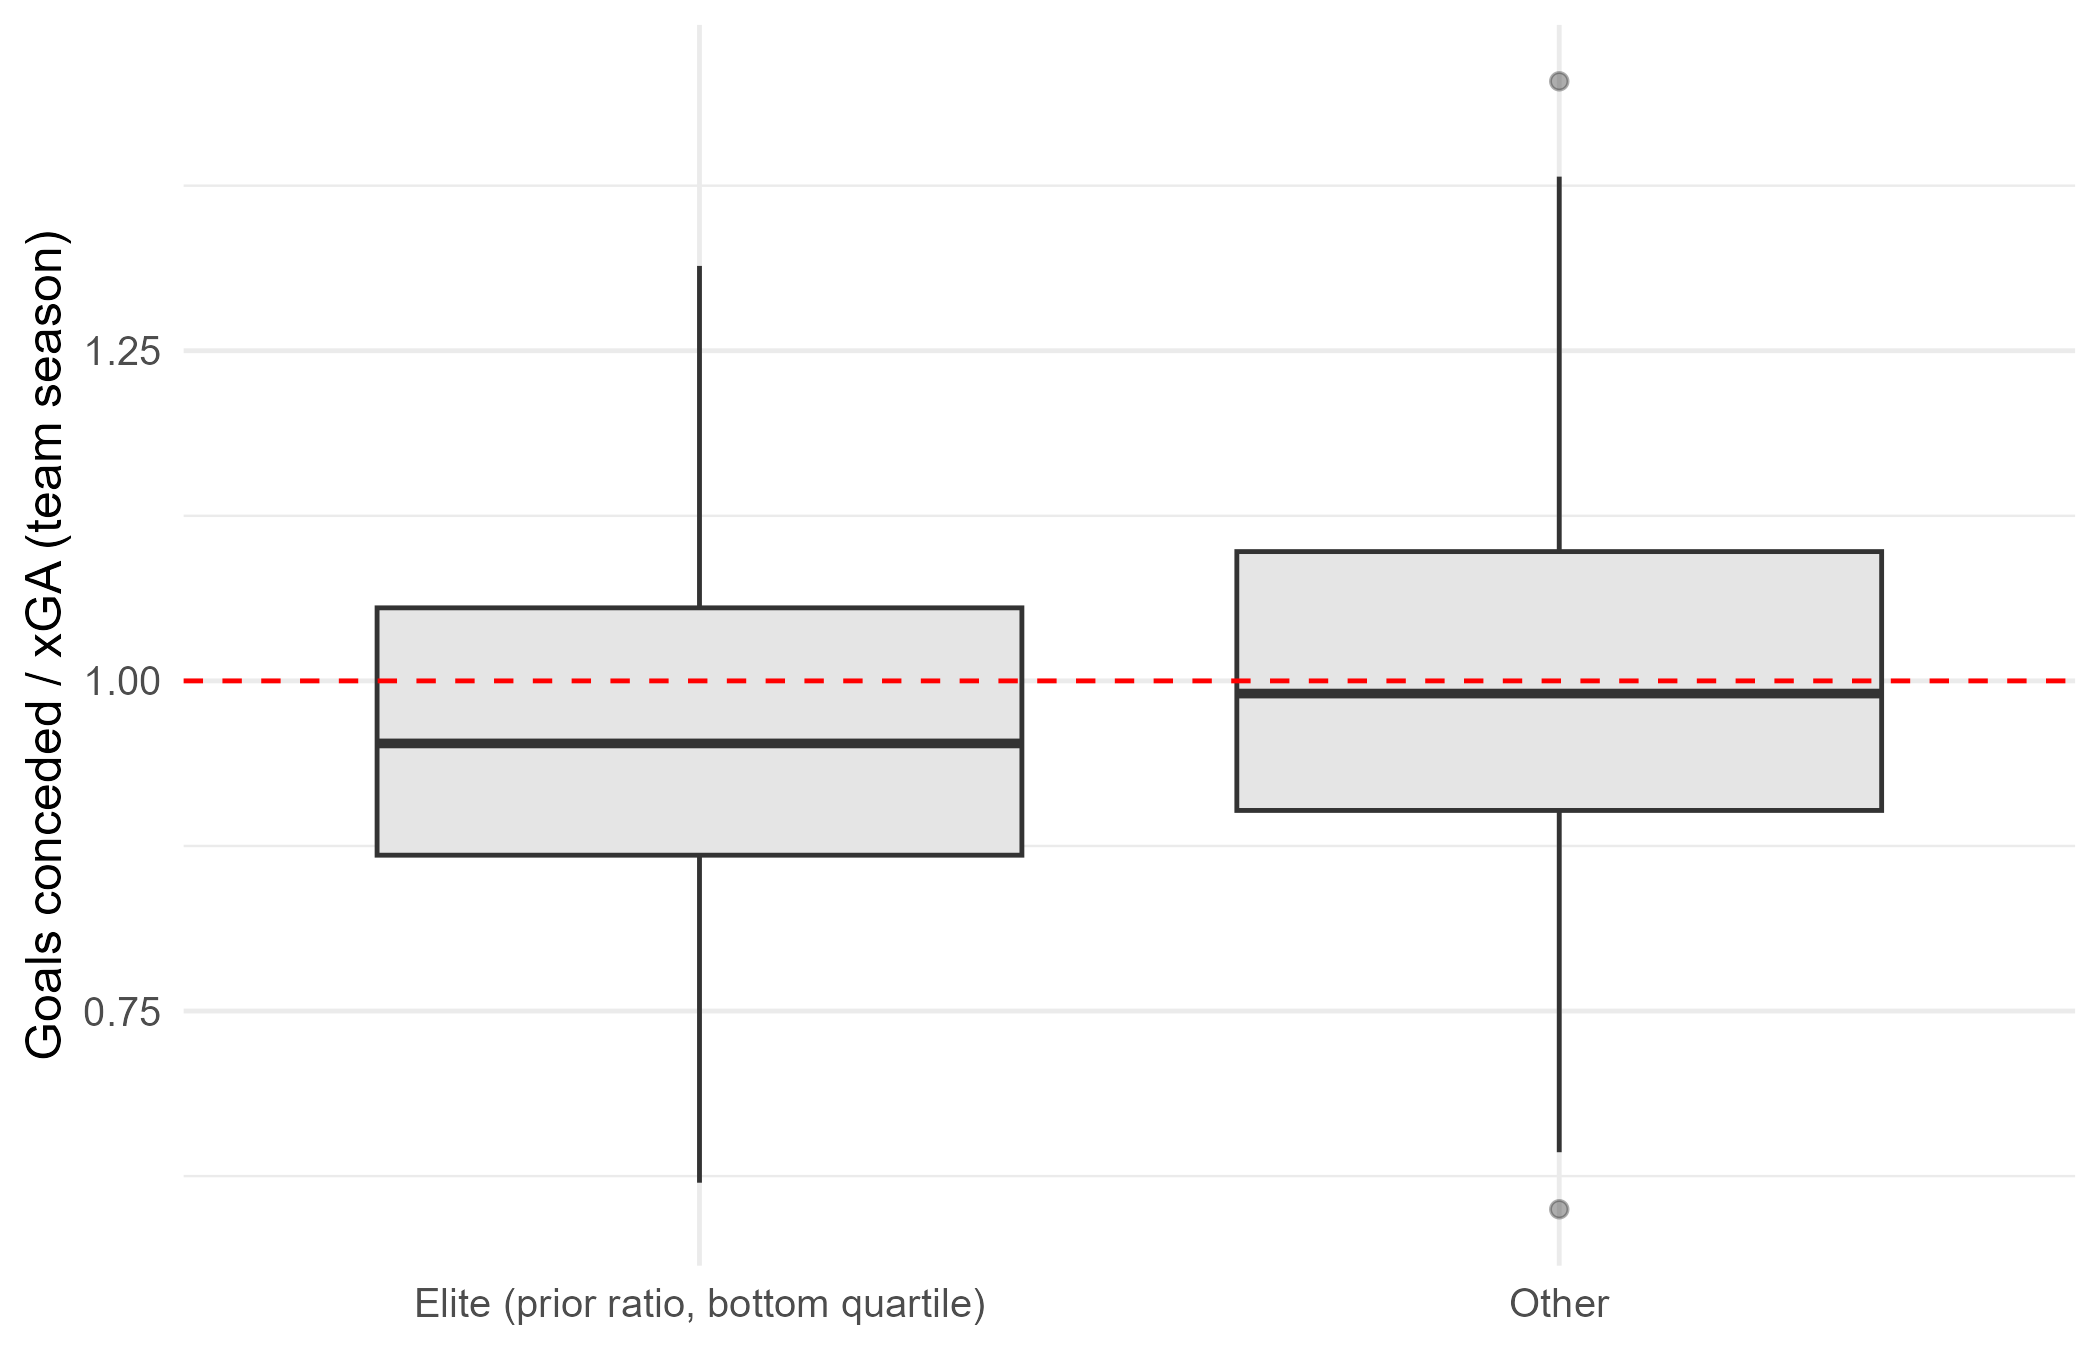
\includegraphics[width=0.6\textwidth]{p2_gk_box.png}
\caption{Goals conceded divided by xGA, by out-of-sample goalkeeper class.}
\label{fig:gkbox}
\end{figure}

\subsection{Regressions and persistence}


\begin{table}
\begin{center}
\adjustbox{max width=\textwidth}{\begin{tabular}{l c c c c}
\toprule
 & (1) goals conceded & (2) ga/xGA, elite & (3) ga/xGA, prior ratio & (4) xGA per match, elite \\
\midrule
xga                     & $1.00^{***}$ &          &             &             \\
                        & $(0.02)$     &          &             &             \\
elite\_num              & $-1.07$      & $-0.02$  &             & $-0.07^{*}$ \\
                        & $(0.61)$     & $(0.01)$ &             & $(0.03)$    \\
prior\_ratio            &              &          & $0.24^{**}$ &             \\
                        &              &          & $(0.08)$    &             \\
\midrule
Num. obs.               & $858$        & $858$    & $858$       & $858$       \\
Num. groups: league     & $6$          & $6$      & $6$         & $6$         \\
Num. groups: season     & $11$         & $11$     & $11$        & $11$        \\
R$^2$ (full model)      & $0.78$       & $0.09$   & $0.10$      & $0.14$      \\
R$^2$ (proj model)      & $0.74$       & $0.00$   & $0.02$      & $0.01$      \\
Adj. R$^2$ (full model) & $0.77$       & $0.07$   & $0.09$      & $0.13$      \\
Adj. R$^2$ (proj model) & $0.74$       & $0.00$   & $0.02$      & $0.01$      \\
\bottomrule
\multicolumn{5}{l}{\scriptsize{$^{***}p<0.001$; $^{**}p<0.01$; $^{*}p<0.05$}}
\end{tabular}}
\caption{Goalkeeper models (goals conceded vs xGA)}
\label{tab:p2_gk_models}
\end{center}
\end{table}

Controlling for xGA and for league and season fixed effects, the elite indicator is associated with about one fewer goal conceded per season (coefficient $-1.07$, $p=0.08$) and a ratio lower by 0.022 ($p=0.11$), borderline significance in regression though clear in the group tests. The prior ratio has a coefficient of 0.24 ($p=0.002$) on next-season ratio: a goalkeeper's past performance predicts about a quarter of the current deviation. The test on the xGA per match shows elite goalkeepers' teams face slightly less dangerous chances (elite $-0.07$, $p=0.04$), suggesting that part of the effect reflects defensive strength or selection into better teams rather than the goalkeeper alone; the data cannot separate these.

\begin{table}

\caption{\label{tab:p2_gk_persistence}Goalkeeper year-to-year persistence (same goalkeeper, seasons t and t+1)}
\centering
\adjustbox{max width=\textwidth}{\begin{tabular}[t]{lrrrrrrr}
\toprule
variable & n\_pairs & pearson\_r & r\_ci\_low & r\_ci\_high & spearman\_rho & slope & slope\_se\\
\midrule
ga\_xga & 625 & 0.187 & 0.110 & 0.261 & 0.180 & 0.189 & 0.040\\
goals\_prevented\_90 & 625 & 0.175 & 0.098 & 0.250 & 0.176 & 0.183 & 0.041\\
xga\_90 & 625 & 0.607 & 0.555 & 0.654 & 0.603 & 0.640 & 0.034\\
\bottomrule
\end{tabular}}
\end{table}

For the same goalkeeper, $\text{ga}/\text{xGA}$ has a year-to-year correlation of 0.19 (CI 0.11--0.26), twice that of forwards' finishing (0.09) but far below the 0.61 persistence of xGA per match. Over long careers, the lowest ratios belong to Oblak (0.82 over 10 seasons), Alisson (0.84), Nick Pope (0.86) and Courtois (0.89) (Table~\ref{tab:p2_gk_career_extremes}), which agrees with their reputations and supports using the ratio as a noisy skill measure.

\begin{table}

\caption{\label{tab:p2_gk_career_extremes}Goalkeepers with the lowest and highest ga/xGA (4+ seasons)}
\centering
\adjustbox{max width=\textwidth}{\begin{tabular}[t]{rlrrrrl}
\toprule
id & player\_name & seasons & ga & xga & ga\_xga & type\\
\midrule
2261 & Jan Oblak & 10 & 297 & 364.214 & 0.815 & Lowest\\
1257 & Alisson & 8 & 280 & 332.710 & 0.842 & Lowest\\
5552 & Nick Pope & 6 & 277 & 321.109 & 0.863 & Lowest\\
7718 & Predrag Rajkovic & 5 & 202 & 230.597 & 0.876 & Lowest\\
680 & Thibaut Courtois & 9 & 307 & 345.998 & 0.887 & Lowest\\
\addlinespace
8858 & Guglielmo Vicario & 4 & 245 & 275.055 & 0.891 & Lowest\\
5652 & Walter Benítez & 5 & 214 & 239.454 & 0.894 & Lowest\\
2415 & David Soria & 7 & 294 & 327.987 & 0.896 & Lowest\\
3503 & Stéphane Ruffier & 6 & 245 & 272.963 & 0.898 & Lowest\\
2090 & Marc-André ter Stegen & 8 & 280 & 310.479 & 0.902 & Lowest\\
\addlinespace
3468 & Jonas Lössl & 5 & 300 & 255.036 & 1.176 & Highest\\
1374 & José Reina & 4 & 155 & 132.956 & 1.166 & Highest\\
2849 & Evgeni Gorodov & 5 & 175 & 154.365 & 1.134 & Highest\\
1328 & Stefano Sorrentino & 5 & 315 & 278.813 & 1.130 & Highest\\
2808 & Sergey Pesjakov & 5 & 199 & 176.415 & 1.128 & Highest\\
\addlinespace
3251 & Paul Bernardoni & 4 & 241 & 214.831 & 1.122 & Highest\\
2072 & Sergio Rico & 4 & 238 & 212.412 & 1.120 & Highest\\
2758 & Anton Shunin & 6 & 207 & 187.409 & 1.105 & Highest\\
2898 & Giorgi Shelia & 4 & 173 & 157.937 & 1.095 & Highest\\
1416 & Ciprian Tatarusanu & 4 & 188 & 173.077 & 1.086 & Highest\\
\bottomrule
\end{tabular}}
\end{table}

\section{Limitations}

\begin{itemize}
\item xG is Understat's own model and not Opta's; results depend on its calibration.
\item Goalkeeper analysis is at the team level: there is no shot-level post-shot xG or save data, so defensive quality and goalkeeping are confounded.
\item ``Elite'' is defined statistically from past performance, not from an external ranking, so it is by construction a noisy proxy.
\item Consecutive-season pairs require both seasons to have $\text{xG}\geq 5$, which excludes injured or benched players.
\item Many tests and specifications are reported; the $p$-values are not adjusted for multiple comparisons.
\end{itemize}

\section{Conclusion}

Multivariate methods lead to a consistent message. xG is well calibrated for forwards, and the extra information in shots is small. Chance creation and volume are stable, individual-level traits (year-to-year correlations of 0.6--0.75), whereas finishing measured by goals/xG is mostly noise within a single season (correlation 0.09) with a small but statistically detectable persistent component. PCA shows that finishing is a separate dimension from creation and volume, and that composite indices describe player profiles well but predict next-season scoring worse than xG per 90 alone. For goalkeepers, the same logic gives a more favorable result: elite goalkeepers selected out of sample do concede fewer goals than xGA (ratio 0.96), a modest effect that is better measured with shot-level data in future work.

\end{document}
